%!TEX root=/Users/sergej/Documents/Thesis-new/main.tex
\section{Empirical results structural RCA}
\label{sec:cross-section}
In this section, I describe the empirical results of the intermediate step of estimating the parameter $\theta$.
Further, I show the results of structural RCA measure.
Further, I analyze the association of the RCA indicator for the three indicators in two steps.
  First, I present the association of structural RCA against GDP plot, which shows whether the association of RCA ranking is related to GDP per capita.
Second, I compare the structural RCA ranking for the country pair Belgium and the Germany across the manufacturing industries.
\par
Table one shows the cross-sectional estimation results for the year 2005.
The columns (2)-(4) report the IV estimates of $\theta$  for different samples regarding the industry coverage and country coverage.
The results show that estimates are robust.
%In the IV estimations, I instrumented the regressor productivity with research and development expenditures as in  \textcite{costinot}.
 First, I note that in both tables as expected the point estimates of $\theta$ are positive and significant.
In column (4) I reduce the sample countries to include only high-income countries based on the world bank classification for 2005.
%\par
%Endogenous trade policy might affect our estimate as follows. First, the econometric error term in the estimation equation 2.1 has a structural interpretation as variable trade cost. Following the outline of \textcite{costinot2010} suppose that a country engages in an endogeneous trade policy which raises the trade barriers based on the penetration of imports. Regarding our regression, this would lead to a correlation of our dependent variable gross exports $\tilde{x}^k_{i,j}$ and the error term $\epsilon_{i,j}^k$. The substation of the relation between policy-induced trade cost and gross exports back into the estimation equation introduces a negative term, which includes the productivity variable, as it was shown analytically in \textcite{costinot2010}. The bias term would introduce a bias of $\theta$ towards zero. Since the EU is a free trade zone a sample only including this countries, is a possibility to control for trade policy effects.
% I report the estimates of the full sample excluding mining and agriculture and the sample excluding only mining.
 %\par
% The OLS estimates for gross exports shows a small yet statistically strongly significant coefficient. The IV estimates in the columns 2-5 are in the range of 15.29 -- 17.64 and are all statistically strongly significant. The estimates show a decreasing pattern between column 2-4. It follows from the interpretation of $\theta$ as the inverse of industry productivity differences that as the parameter is smaller in column (3) than in column (2)  that the sample excluding agriculture and mining shows a higher cost dispersion compared to the full sample. The cost dispersion in the service and manufacturing industries in the sample is higher than the agriculture and mining industry. Moreover, since the estimate of $\theta$ is smaller in column (4) than in column (3) I conclude that agriculture shows a higher cost dispersion than mining. Also, comparing column (5)with column (1) shows that endogenous trade protection does not significantly bias the estimate of $\theta$, as the estimate in column (5) is in the 95\% interval of column (1). The differences in $\theta$ between both tables in the same columns are not significant.
\par
The OLS estimates for gross exports, and backward value-added exports show a small yet statistical strongly significant coefficient.
 The IV estimates in the columns (2)-(4) are significantly increased with an estimated $\theta$ between 12.63 and 14.68.
 I interpret the increase of the IV estimate as an indicator that the independent variable is endogenous since otherwise, both estimates should show no significant difference \textcite{hausman1978}.
From a substantial point of view, there are mainly two reasons, why I use an instrument to account for the potential endogeneity of $\tilde{z}^k_i $.
First, the estimates of $\theta$ might be biased because of measurement error in the international price data.
The measurement error would bias the estimate towards zero \parencite{AngristKrueger01}.
%If an explanatory variable is measured with additive
%random errors, then the coefficient on that variable in a bivariate ordinary least
%squares regression will be biased toward zero in a large sample. The higher the
%proportion of variability that is due to errors, the greater the bias. Given an
%instrument that is uncorrelated with the measurement error and the equation error
%(that is, the equation error from the model with the correctly measured data), but
%correlated with the correctly measured variable, instrumental variables provide a
%consistent estimate even in the presence of measurement error.
%Another reason, may be that agglomeration effects cause a simultaneity bias  \parencite{costinot}.
%An agglomeration effects as e.g. that firms locate geographically close to each other and learn about exports opportunities.
%This creates a link from higher export levels to increased the productivity.  %\par
%The IV regression requires that the instrument is valid, which means that it satisfies the exclusion restriction and that it is relevant.
 %The exclusion restriction requires that the instrument R\& D has no explanatory power for exports except through productivity.
  %The restriction is plausible  \textcite{costinot} showed that for their sample the estimates of $\theta$ were not sensitive, to changes in productivity as total factor productivity.
  % The interpretation is that the variations of the prices, which are explained by R \& D are orthogonal to factor endowment trade motifs.
\par   The results of the first stage regression address two concerns about the validity of the IV regression, first the relevance of the instrument and whether the causal effect of the instrument is as expected.
Firstly, concerning the relevance of the instrument, the table (see appendix) shows the F-statistic of the excluded instrument in the first stage is across the specifications very high and hence the instrument is highly relevant.
Further, the first stage shows a statistically significant positive effect of  R\&D on the inverse of producer prices, which confirms the hypothesis of a positive causal effect of R\&D on the producer prices.  %Further, to gauge the relevance I comparing the magnitude of the effect of R\& D on the inverse of producer prices to  the results of the authors \textcite{costinot}, I find that the effect of R\&D on producer prices is 42 percent lower in my sample \footnote{The estimated effect of R\& D on the inverse of producer prices is 0.038 with an standard error of 0.003 in the sample of \textcite{costinot} . The estimate in my full sample is only 0.022 with an SE of 0.002. } . Since the IV estimator for one instrument may be obtained by the reduced form coefficient scaled by the first stage estimate, the reduced coefficient of the first stage likely accounts partly for the increased estimate of $\theta$ in direct comparison. I conclude that statistically the estimates are not weakly identified, and diagnostic plots of the residuals against the fitted values do not suggest misspecification. However, the magnitude of the estimates is compared to the directly obtainable
 \par
The IV estimates of $\theta$  show following results.
 First, the comparison between the full and the sample excluding primary industries shows that the estimates are similar for $\theta$ for both backward value-added and gross exports.
 In general comparing the estimates of $\theta$ for both dependent variables, I conclude that the estimates are statistically not significantly different.
 Second, the pattern for both dependent variables shows that the estimate from the sample excluding the primary industries is statistically not significantly decreased.
 Third, the sample excluding no high-income countries and primary industries shows a statistically significantly increased estimate compared to the full sample \footnote{Based on an extension of the t-test to the multiple imputation setting.
  The distribution of test statistic is a t-distribution with $v$ degrees of freedom, where $v=(m-1)*(1+ ((1+M{-1})*B/ \bar{U}){-1})^2$ and $\bar{U}$ denotes the average within-imputation variance and $B= 1/m-1*\sum_i=1^m \theta_i-\bar{\theta})$ denotes the between imputation variation of the estimated parameter \textcite[p.77]{Rubin1987}}.
   %The magnitude of the increase of $\theta$ is about  28 \%.
From a substantial point, a higher point estimate of $\theta$ implies a decreased dispersion.
The effect is expected, as the sample includes only high-income countries.\par
The table for the dependent variable forward value-added exports shows noticeable differences.
In the first column, the OLS estimate shows a negative sign and is not significant.
The negative sign of the OLS estimate may be caused by bias.
However, since the OLS estimate is not significant, I forgo a further discussion.
The IV estimates for the different samples are statistically significant and show positive estimates.
Surprisingly, the estimate for the last sample, which includes only high-income countries, is not increased.
Overall the estimates for forward value-added exports are very stable and change little across the different samples.
  \par
  Compared to \textcite{costinot} I find that the estimates without primary industries, which is the closest matching sample, show comparable estimates.% e.g  ($\theta$11.1 SE 0.981).
   However, the authors best estimate of 6.58 is significantly lower than the results I obtained.
   The authors obtained the estimate with the dependent variables openness corrected gross exports.
  They argued that openness corrected gross exports are necessary to account for trade selection \footnote{ Trade selection denotes that a country does not produce certain goods for which they receive a low productivity draw and instead imports them (\cite{costinot}).}
    downward biases the differences in observed productivity compared to the fundamental productivity.
     Therefore, they reasoned that the estimates of  $\theta$ with gross exports are upward biased. \par
    In this thesis, I use gross exports and value added exports without an openness correction.
     First, the authors used the import penetration ratio to correct for openness.
     This measure is only available for the manufacturing industries and hence applying the correction would reduce my sample coverage.
      Second, it is not clear, how to correct for openness for the dependent variable value-added exports  \footnote{ A possible definition openness for value-added exports might be the ratio of re-imported value added from domestic industries to value-added exports .
      However,  the estimates of $\theta$ with this correction showed implausible values.}.
\begin{table}[H]
\caption{Cross-section Results OLS and IV}
\scriptsize
\begin{savenotes}
\begin{subtable}{0.9\textwidth}
\centering \caption{Cross-section results I}
\label{tab:EXGR}
{
\def\sym#1{\ifmmode^{#1}\else\(^{#1}\)\fi}
\begin{tabular}{l*{4}{S}}
\toprule
            &\multicolumn{1}{c}{(1)}&\multicolumn{1}{c}{(2)}&\multicolumn{1}{c}{(3)}&\multicolumn{1}{c}{(4)}  \\ %& %\multicolumn{1}{c}{(5)}
            &\multicolumn{1}{c}{OLS}&\multicolumn{1}{c}{Full Sample}&\multicolumn{1}{c}{Without primary}& \multicolumn{1}{c}{Without primary} \\
        & \multicolumn{1}{c}{}    & &\multicolumn{1}{c}{industries} & \multicolumn{1}{c}{industries high \footnote{\footnotesize denotes highly developed countries, in the sample this includes the following countries AUS, AUT  BEL, CAN\\
CZE, DEU, ESP, EST, FIN, FRA, GBR, GRC, HUN, IRL, ITA, JPN, KOR, LUX, NLD, POL, PRT, RUS, SVK, SVN, USA} } %\\&\multicolumn{1}{c}{EU}
            \\ \midrule
                        \multicolumn{5}{c}{Dependent variable log gross exports in 2005} \\
\midrule
Log productivity&     0.43368 &     12.653 & 11.424 & 14.689  \\
& (0.067) & (1.331) & (1.422) & (2.13) \\

% 0.43\sym{***}&        15.97296\sym{***}&       16.66\sym{***}&     19.13\sym{***} \\%&       17.19\sym{***}\\
%            &      (0.07)         &      (.3127033)         &      (1.99)         &       (2.52)         &
       %\\%     (2.19)         \\
\midrule

Exporter-Importer Fixed Effects & \multicolumn{1}{c}{YES}&\multicolumn{1}{c}{YES}&
\multicolumn{1}{c}{YES}%&\multicolumn{1}{c}{YES}
 &\multicolumn{1}{c}{YES}\\
 Importer-Industry Fixed Effects& \multicolumn{1}{c}{YES}&\multicolumn{1}{c}{YES}&
 \multicolumn{1}{c}{YES}&\multicolumn{1}{c}{YES} \\%&\multicolumn{1}{c}{YES}\\
\midrule
Observations     &        \multicolumn{1}{c}{18143 }        &     \multicolumn{1}{c}{18143  }        &      \multicolumn{1}{c}{16582}         &      \multicolumn{1}{c}{14449}        \\% &       \multicolumn{1}{c}{9678 }         \\
 R-squared* & 0.771& 0.197 & 0.321 & 0.141\\
First-stage F-statistic exc. instrument    &        &  151.41&     125.60      &      85.24                \\\bottomrule% &
   %  68.54         \\\bottomrule
\multicolumn{5}{l}{\footnotesize Heteroscedasticity robust standard errors in parentheses}\\
\multicolumn{5}{l}{\footnotesize Log Productivity is instrumented in columns 2-4 with log of R\&D expenditures}\\
\multicolumn{5}{l}{\footnotesize Without primary industries excludes the industries agriculture and mining} \\
\multicolumn{5}{l}{*  avg. of imputed R-squareds}\\
\end{tabular}
}
\end{subtable}
\begin{subtable}{0.9\textwidth}
\scriptsize
\centering \caption{Cross-section results II}
\label{tab:EXGR-DVA}
{
\def\sym#1{\ifmmode^{#1}\else\(^{#1}\)\fi}
\begin{tabular}{l*{4}{S}} \toprule
      &\multicolumn{1}{c}{(1)}&\multicolumn{1}{c}{(2)}&\multicolumn{1}{c}{(3)}&\multicolumn{1}{c}{(4)}  \\
      %&\multicolumn{1}{c}{(5)}
                      &\multicolumn{1}{c}{OLS}&\multicolumn{1}{c}{Full Sample}&\multicolumn{1}{c}{Without primary}& \multicolumn{1}{c}{Without primary} \\
        &   &  & \multicolumn{1}{c}{industries} & \multicolumn{1}{c}{industries high}\\ \midrule
                               \multicolumn{5}{c}{Dependent variable log backward value-added exports in 2005} \\ \midrule
 Log Productivity&   0.476 & 12.911 & 11.762 & 15.080 \\
   &( 0.066) & (1.340) & (1.447) & (2.180) \\
%            &      (0.07)         &      (1.78)         &      (2.01)         &      (2.54)
%           \\%    (2.17)         \\

Exporter            Importer Fixed Effects & \multicolumn{1}{c}{YES}&\multicolumn{1}{c}{YES}&\multicolumn{1}{c}{YES}&\multicolumn{1}{c}{YES}% &\multicolumn{1}{c}{YES}
\\
 Importer Industry Fixed Effects & \multicolumn{1}{c}{YES}&\multicolumn{1}{c}{YES}&\multicolumn{1}{c}{YES}&
\multicolumn{1}{c}{YES} \\ \midrule %&\multicolumn{1}{c}{YES}\\\midrule
Observations     &        \multicolumn{1}{c}{18085}         &       \multicolumn{1}{c}{  18085 }         &     \multicolumn{1}{c}{  16538 }        &      \multicolumn{1}{c}{  14412 }      \\
%  &        \multicolumn{1}{c}{  9659 }      \\
  R-squared* &  0.775 & 0.180 & 0.304 & 0.128 \\
%F-statistic second stage &         50.68        &       54.56        &       60.05        &   60.82
   % \\%  63.94        \\
%Kleibergen-Paap rk Wald F-statistic&                      &  109.81         &       85.94         &     68.84
First-stage F-statistic of exc. instrument &  &151.41&     125.60      &      85.24           \\
    \bottomrule %     70.78      \\
\multicolumn{5}{l}{\footnotesize Heteroscedasticity robust standard errors in parentheses}\\
\multicolumn{5}{l}{\footnotesize Log Productivity is instrumented in columns 2-4 with log of R\&D expenditures}\\
\multicolumn{5}{l}{\footnotesize Without primary industries excludes mining and agriculture industry} \\
\multicolumn{5}{l}{* avg. of imputed R-squareds}\\
\end{tabular}
}
\end{subtable}
\begin{subtable}{0.9\textwidth}
\scriptsize
\centering \caption{Cross-section results III}
\label{tab:EXGR-FDDVA}
{
\def\sym#1{\ifmmode^{#1}\else\(^{#1}\)\fi}
\begin{tabular}{l*{4}{S}} \toprule
      &\multicolumn{1}{c}{(1)}&\multicolumn{1}{c}{(2)}&\multicolumn{1}{c}{(3)}&\multicolumn{1}{c}{(4)}
        \\%&\multicolumn{1}{c}{(5)}
                    &\multicolumn{1}{c}{OLS}&\multicolumn{1}{c}{Full Sample}&\multicolumn{1}{c}{Without primary}& \multicolumn{1}{c}{Without primary} \\
        &   &  & \multicolumn{1}{c}{industries} & \multicolumn{1}{c}{industries high}\\ \midrule
                                    \multicolumn{5}{c}{Dependent variable log forward value-added exports in 2005} \\ \midrule
           %  \\ \midrule
 Log Productivity&          -0.0191         &  9.286 & 10.325 & 10.218  \\%   0.476 & 12.911 & 11.762 & 15.080 \\
            &      (0.0454)        &(0.868) & (1.291) & (1.199) \\ %     (1.15)         &      (2.05)         &      (1.94)         \\%&      (1.39)         \\
Exporter   Importer Fixed Effects & \multicolumn{1}{c}{YES}&\multicolumn{1}{c}{YES}&\multicolumn{1}{c}{YES}&
\multicolumn{1}{c}{YES} \\ %&\multicolumn{1}{c}{YES}\\
 Importer Industry Fixed Effects & \multicolumn{1}{c}{YES}&\multicolumn{1}{c}{YES}&\multicolumn{1}{c}{YES} &\multicolumn{1}{c}{YES}
 \\ \midrule
Observations     &        \multicolumn{1}{c}{16727}     &        \multicolumn{1}{c}{16727}         &        \multicolumn{1}{c}{15271}         &        \multicolumn{1}{c}{14095}       \\ %/         %\multicolumn{1}{c}{8918}         \\
R-squared* &        0.882 & 0.475 & 0.431 & 0.488     \\  %&       83.89         \\
First-Stage F-statistic of exc. instrument&                       &     151.41&     125.60      &      85.24           \\     %&       96.01         \\
\bottomrule
\multicolumn{5}{l}{\footnotesize Heteroscedasticity robust standard errors in parentheses}\\
\multicolumn{5}{l}{\footnotesize Log Productivity is instrumented in columns 2-4 with log of R\&D expenditures}\\
\multicolumn{5}{l}{\footnotesize Without primary industries excludes the industries mining and agriculture} \\
\multicolumn{5}{l}{* avg. of imputed R-squareds}\\
\end{tabular}
}
\end{subtable}
\end{savenotes}
\end{table}

In the following, I discuss the results of the structural RCA ranking for both value-added exports measures and gross exports.
Especially, I will show two applications of the structural RCA ranking.
First, I show a scatter plot of the association of the RCA ranking for gross exports and value-added exports and a country's GDP per capita.
The plot is used to analyse the hypothesis that countries with a higher GDP show a greater similarity between the rankings.
The reason may be that more developed countries use the production factors in a less sector-specific manner. \par
The second application compares the structural RCA ranking for Belgium and Germany based on forward and backwards value-added exports and gross exports.
By analysing the pattern of RCA for a country pair, it can be directly seen whether value-added exports change the conclusions about a country's comparative advantage.
Moreover, I research whether both perspectives show a similar story about countries comparative advantage industries.
\subsection{Structural Ricardian comparative advantage based gross exports and value-added exports}
To compare the RCA rankings I have chosen the following association.
First of all, I chose the Spearman's $\rho$  since I focus on the similarity of the rankings.
Moreover, I chose Kendall's $\tau$ as it computes the similarity of the two rankings, by counting the number of country pairs, which are different between two rankings.
Also, Kendall's  $\tau$ may be interpreted as the difference between the probability of concordance and discordance of two variables \parencite{newson2parameters}.
Finally, both measures are invariant to any rescaling of the ranking variable, which preserves the ordering of the countries.
The property is useful, as the estimates of $\theta$ are in the upper range of previous results.
\par
% I outline the construction of Kendall's $\tau$ based on \textcite{abdi2007kendall}.
% The outline makes the simple interpretation of Kendall's $\tau$ in terms of probabilities more clear.
% The basic idea behind the measure is to count the number of different pairs of two sets of ordered  objects, which include the same objects  \textcite{abdi2007kendall}.
% I illustrate this idea in the context of the RCA rankings.
% For two RCA rankings, the measure is based on counting the number of different ordered country pairs, which I denote as $d(P_1, P_2)$, where $P_i \quad i=1,2$ indicates the two ordered set of pairs obtained from the country rankings.
% In the next step, this number is normalized such that is bounded by -1 and 1, where -1 reflects the largest differences and 1 is equal to the smallest difference.
% Kendall's $\tau$ is then defined as follows \[ \tau= \frac{1/2 N(N-1) - d(P_1,P_2)} {1/2 N(N-1)} .\] %where the nominator $1/2 N(N-1)$ is equal to the number of pairs one can obtain from a set of $n$ objects.
% Moreover, Kendall's $\tau$ has an intuitive stochastic interpretation based on the idea of drawing ordered pairs \parencite{abdi2007kendall}.
% In the context of two country rankings, the interpretation is that if a country pair is randomly drawn from each ranking, Kendall's $\tau$ is the difference between the probability that the draws have the same order and the probability that the country pairs have a different order.
% The focus of Kendall's $\tau$ on country pairs is especially useful for RCA, as the main focus of RCA is to compare pairs of countries and industries.   \par
\begin{figure}[H]
\caption{Association RCA based on VAX \& EXGR and GDP per capita }
\centering
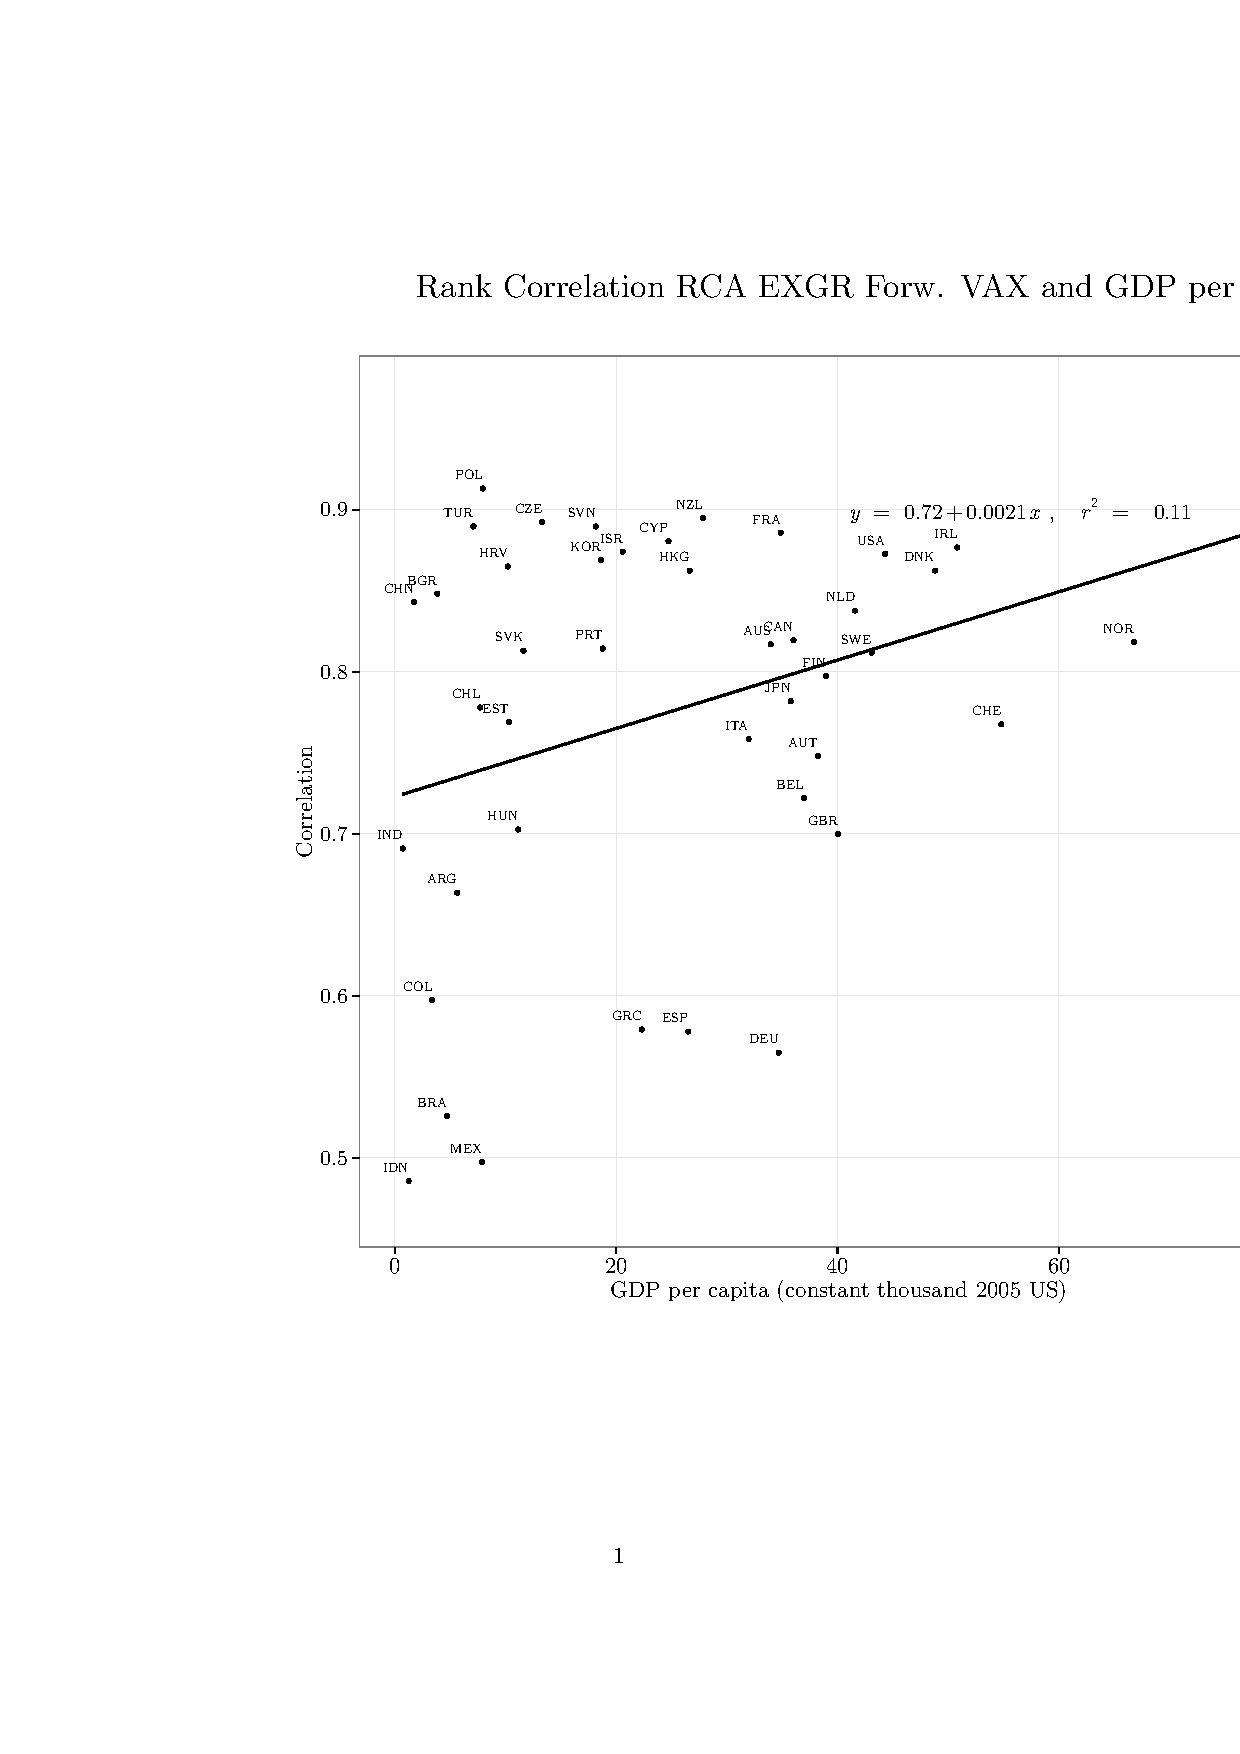
\includegraphics[width=.49 \linewidth]{./fig/spearman_fddva_std_balassa-march.tex}
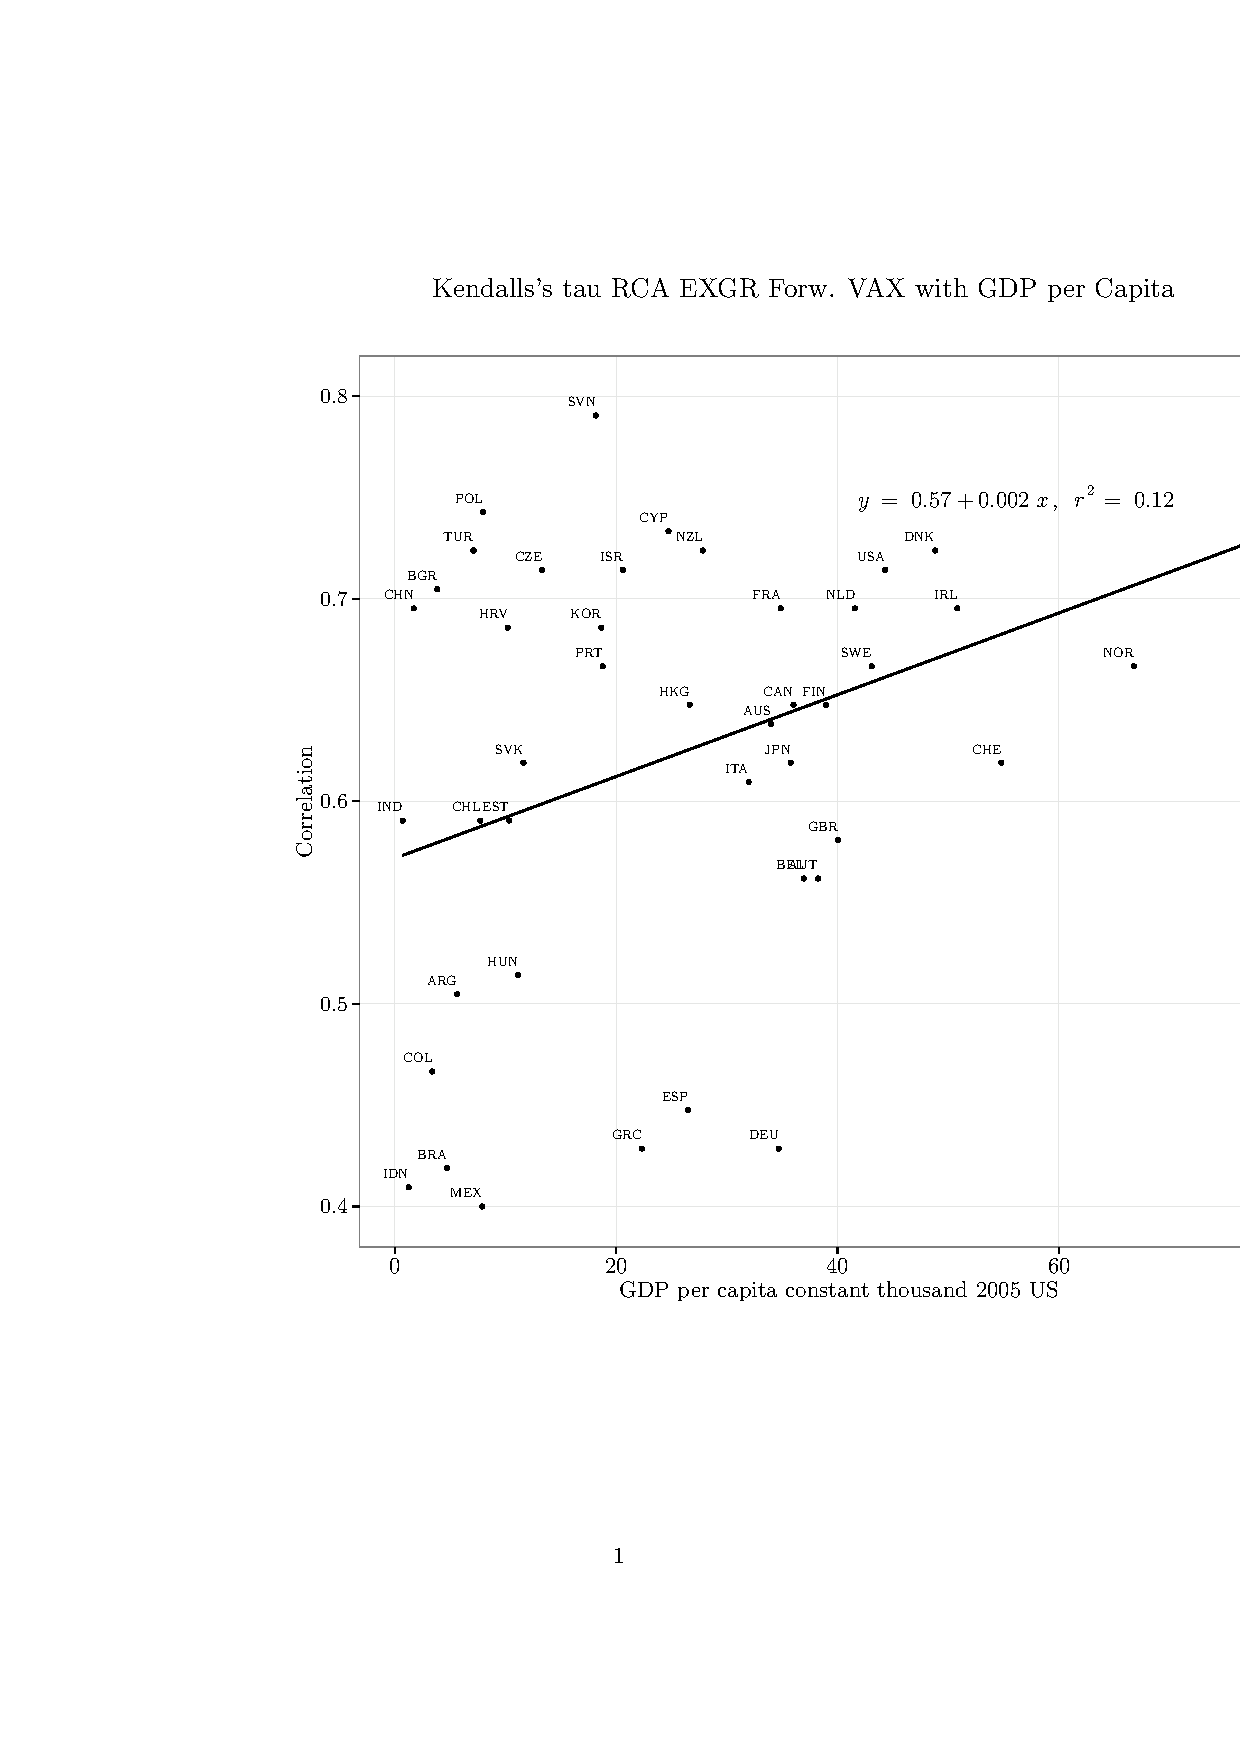
\includegraphics[width=.49\linewidth]{./fig/kendall_fddva_exgr_std_balassa-march.tex}
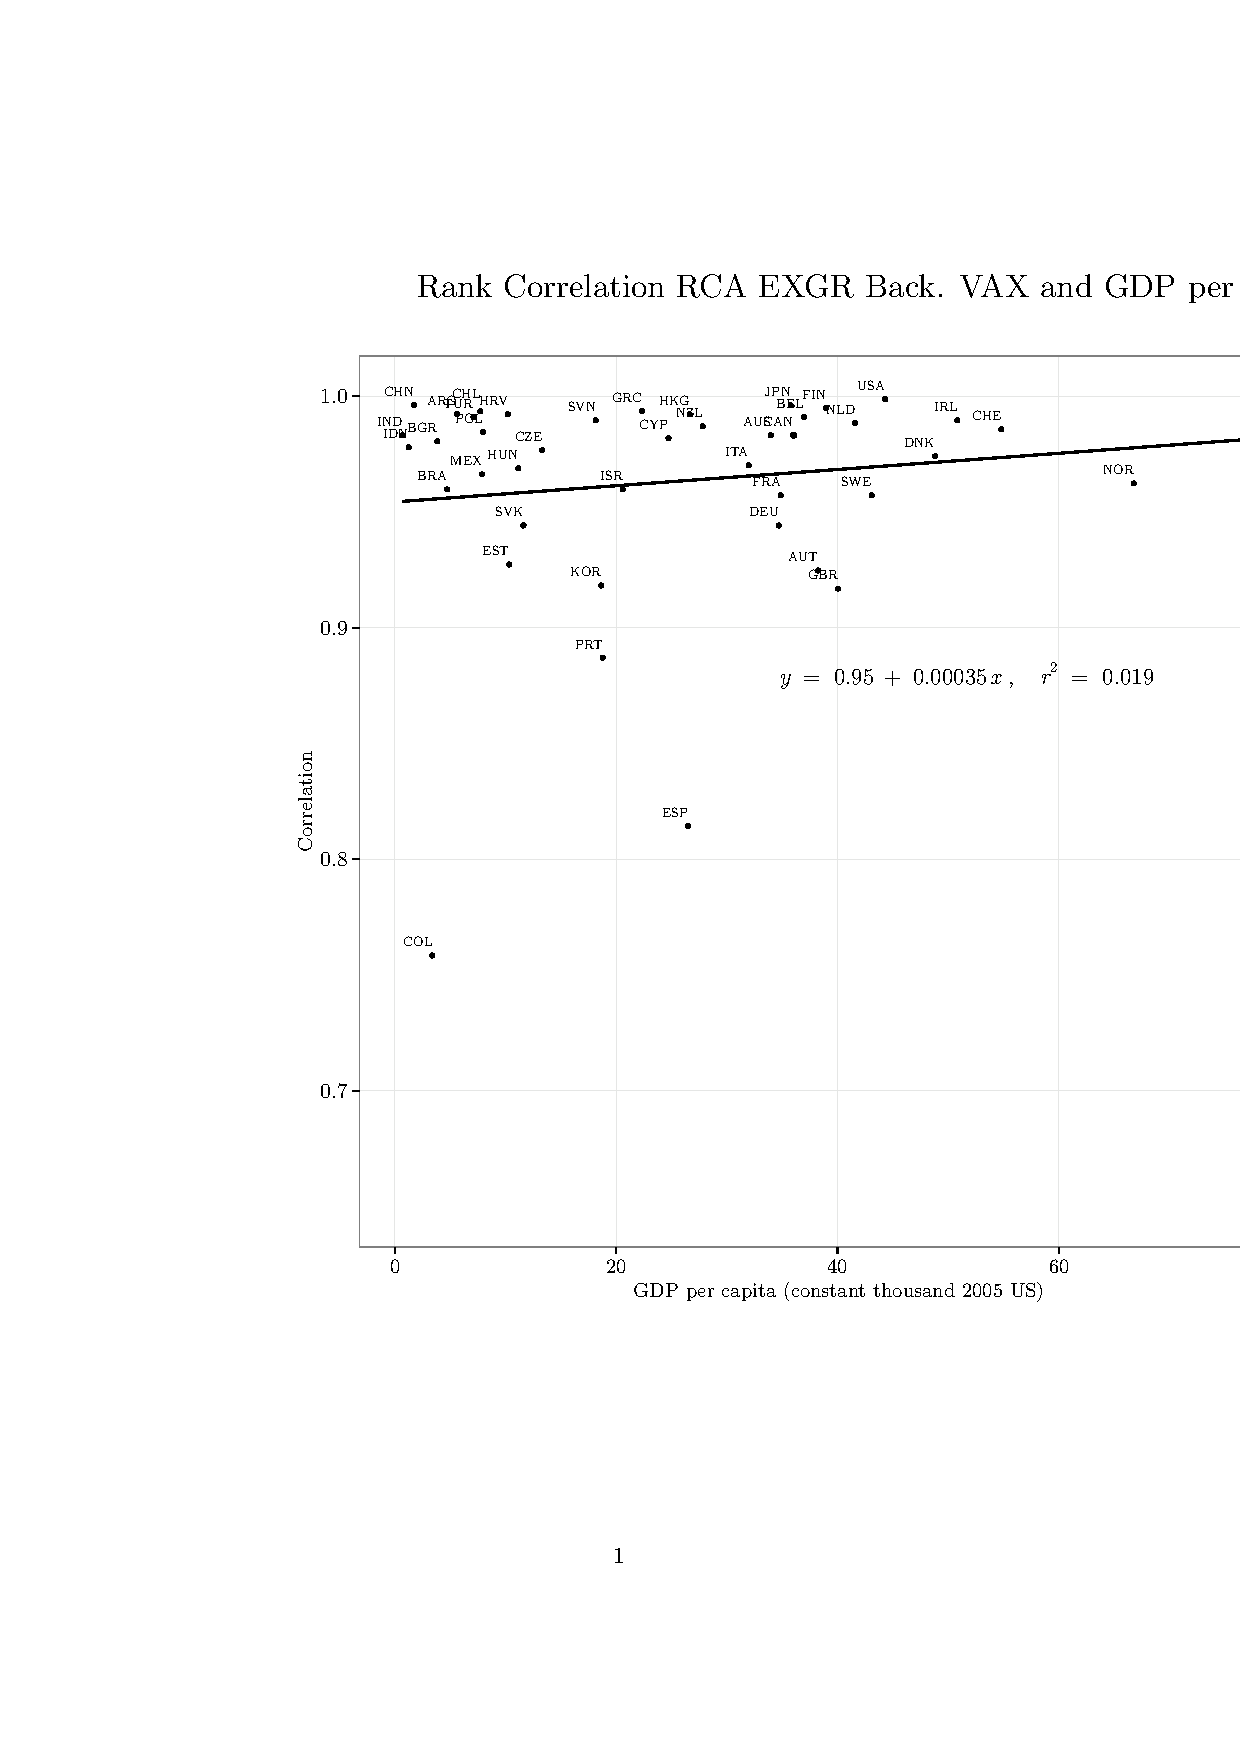
\includegraphics[width=.49 \linewidth]{./fig/spearman_exgr_dva_std_balassa-march.tex}
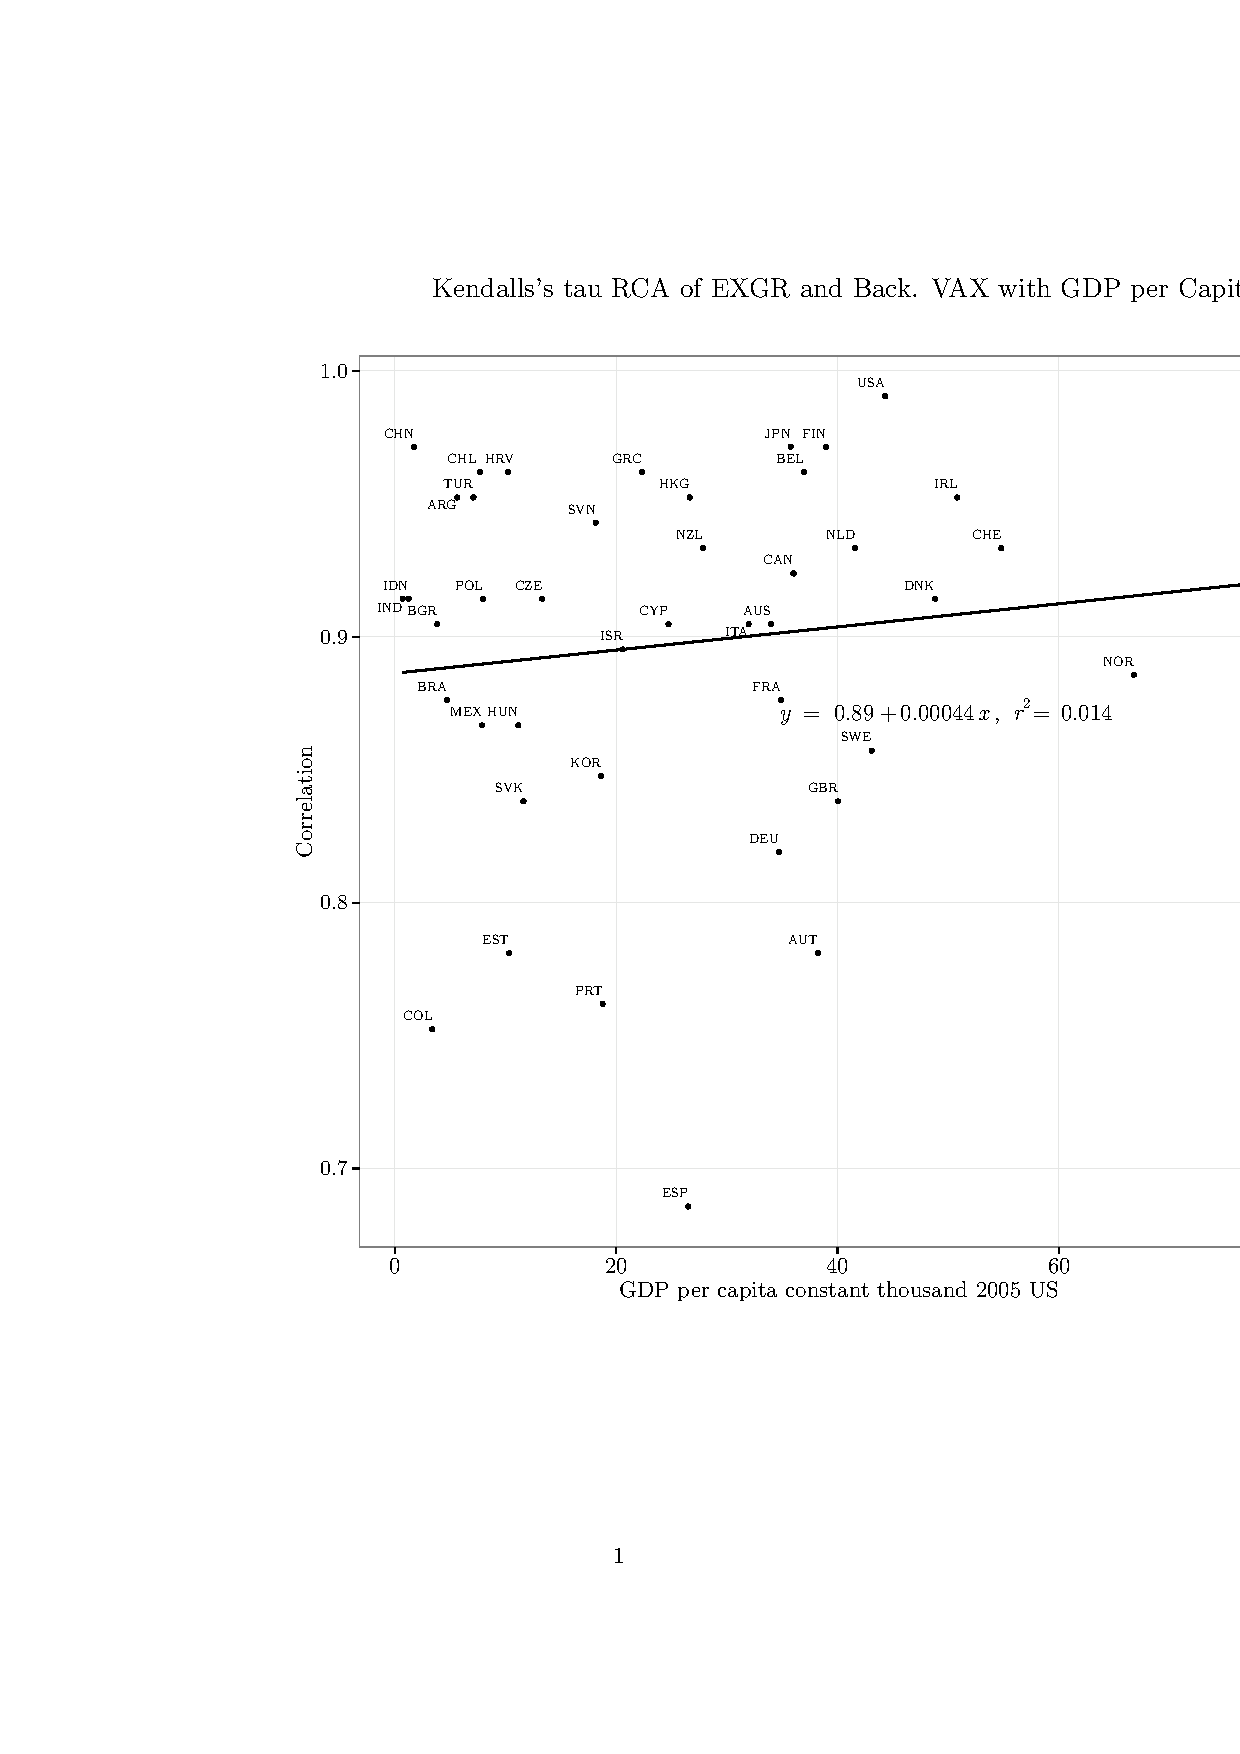
\includegraphics[width=.49\linewidth]{./fig/kendall_dva_exgr_std_balassa-march.tex}
 %\captionof{figure}{Another figure}
\end{figure}
I conclude four findings from the figures above.
Firstly, the RCA rankings based on gross exports and backward value-added exports show a high degree of similarity for all countries.
Secondly, the association between forward value-added exports and gross exports is substantially lower than the association of backwards value-added and gross exports.
Thirdly,  the association of gross exports and forward value-added exports  show a weak positive association with a country's GDP per capita.
However, the positive relation in the graph is not robust to the exclusion of the country with the lowest and the highest RCA from the graph. Such a change would alter the graph to a flat line.
As a final point, I find that the overall strength of the associations is higher using  Spearman's $\rho$ compared to Kendall's $\tau$. \par
The first and second finding are similar to the results in the estimation of the $\theta$ parameter, which showed similar estimates using gross exports and backward value-added exports while the estimates using forward value-added exports showed differences.
The finding of a smaller association for Kendall compared to Spearman is unsprising, given that the population analog of Spearman's $\rho$ and Kendall's $\tau$ is equal to three half \parencite{fredricks2007}. \par
The country pair graph comparing RCA for the three indicators backward/forward value-added exports and gross exports present a more local view of RCA.
 below I present  the normalized RCA based on both value-added export measures and gross exports for the industries of the manufacturing sector.
the RCA \footnote{ Formally, I define it as follows $RCA_{i}^{k}=\frac{ z^k_i * \bar{z} }{\bar{z}_i * \bar{z}^k}$, where $\bar{z}=1/NK* \sum_{i=1}^N \sum_{k=1}^K z^k_i$ denotes the grand mean, $\bar{z}^k= 1/N \sum_{i=1}^N z^k_i$ denotes the industry specific mean and $\bar{z}_i= 1/K \sum_{k=1}^K z^k_i$ denotes the country specific mean.} as in \textcite{leromain2014}.
The normalized RCA has the following interpretation, a value above (below) one indicates a comparative (dis)advantage of a country in a specific industry.
 \par
 To start with the RCA ranking results, I discuss the results for backward value-added exports and gross exports.
 I find that for both countries backward value added closely traces the RCA pattern of gross exports.
\par
 The figure highlights that both countries highlights have a comparative advantage in the following industries wood industry (ISIC Rev.3 20), fuel products (ISIC Rev. 3, 23), chemical (ISIC Rev. 3 24) and other non-metalic mineral products (ISIC Rev. 3 26).
 Germany has a higher comparative advantage in seven industries namely the wood industry, paper and printing(ISIC. Rev. 3 21-22), rubber and plastics (ISIC Rev. 3, 25), basic metals and metal products (ISIC Rev. 3, 27-28), machinery and equipment (ISIC Rev. 3, 29), electrical and optical equipment (ISIC Rev. 3, 30-33) and transport equipment (ISIC Rev.3, 34-35).
 On the other hand, Belgium has a higher comparative advantage in six industries namely the food industry (ISIC Rev. 3 15-16), textiles, leather and footwear industry (ISIC Rev.3, 17-19), fuel products, chemical, manufacturing and recycling (ISIC Rev. 3 ,36-37).
  \par
 In contrast, the RCA rankings based on forward value-added gross exports show larger differences .
 The figure shows the largest decrease of RCA in the industries paper products (ISIC. Rev. 3, 21) and wood (ISIC. Rev. 3 20).
 Additionally Germany shows a large decrease of RCA for the paper and printing products industry .
 The largest decrease of RCA induces a change of 15\%  in the industry chemical products industry (ISIC. Rev. 3 23) for both countries.
 As a result, the  chemical products industry  changes from a comparative advantage to an industry of comparative disadvantage for Germany.
 %The industry changes from a comparative advantage to comparative disadvantage, whereas for Belgium the industry remains a comparative advantage.
 Additionally, in wood industry both countries  no longer show a comparative advantage under forward  value-added exports whereas under gross exports they show a comparative advantage.
 Moreover, I observe the largest increase of RCA under forward value-added exports compared to gross exports in the industry 29 and 30-33.
 For both countries, I observe an increase of about 5\% in the industry 30-33 for forward value-added exports and a somewhat smaller increase in the industry 29.
 However, the pattern of RCA remains unchanged for both countries, for Belgium, a comparative disadvantage and Germany has a comparative advantage.
 Concluding, the graphical analysis show that forward value-added exports changes the pattern of RCA, whereas the RCA pattern under backward value-added exports and gross exports is similar.
 \begin{figure}
\caption{Comparative advantage based on for- and backward  VAX \& EXGR for Belgium and Germany}
\includegraphics[width=.5\linewidth]{./fig/forw_exgr_DEU_BEL_tiva.tex}
\includegraphics[width=.5\linewidth]{./fig/back_exgr_DEU_BEL_tiva.tex}
\end{figure}
\endinput
